\documentclass{article}

\usepackage{graphicx}
\usepackage{subcaption}
\begin{document}
	
	\section{Side-by-Side Images}
	
	Figure \ref{fig:comparison} shows two images placed next to each other.
	
	\begin{figure}
		\centering
		
		\begin{subfigure}{0.45\textwidth}
			\centering
			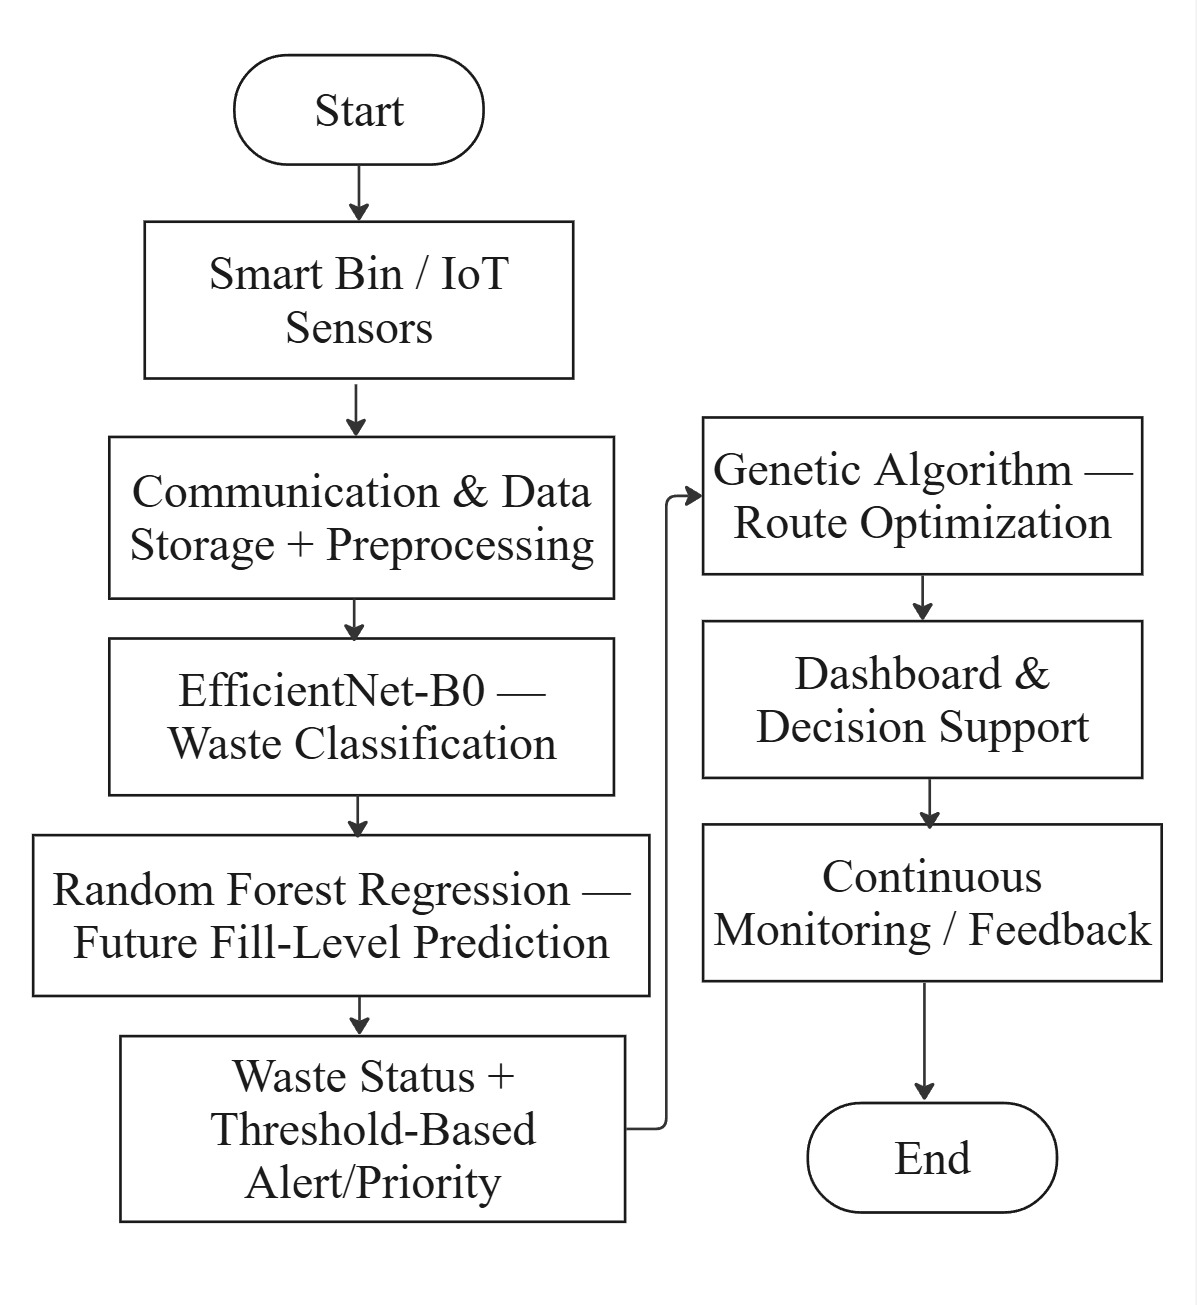
\includegraphics[width=\textwidth]{flow.jpg}
			\caption{First image}
		\end{subfigure}
		\hfill
		\begin{subfigure}{0.45\textwidth}
			\centering
			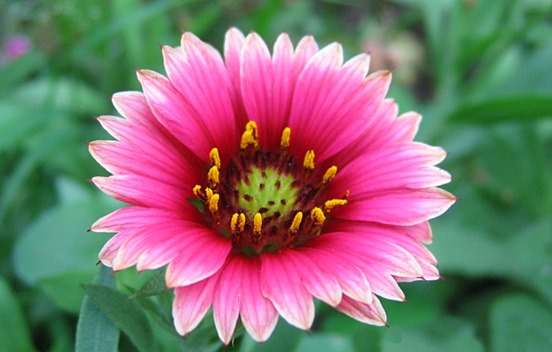
\includegraphics[width=\textwidth]{flower.jpg}
			\caption{Second image}
		\end{subfigure}
		
		\caption{Comparison of two images}
		\label{fig:comparison}
		
	\end{figure}
\end{document}